\documentclass[tikz,border=7pt]{standalone}
% Shared visual language for the book's standalone vector figures.
% Keep this file compatible with the TeX Live version used by LyX.
\usepackage{amsmath,amssymb}
\usepackage{array,booktabs}
\usepackage{pgfplots}
\usepackage{pgfplotstable}
\usetikzlibrary{arrows.meta,calc,positioning}
\pgfplotsset{compat=1.17}

\definecolor{BookBlue}{HTML}{0072B2}
\definecolor{BookOrange}{HTML}{D55E00}
\definecolor{BookGreen}{HTML}{009E73}
\definecolor{BookGray}{HTML}{666666}
\definecolor{BookLightGray}{HTML}{D9D9D9}

\pgfplotsset{
  book axis/.style={
    axis line style={black!75,line width=0.55pt},
    tick style={black!75,line width=0.45pt},
    tick label style={font=\small},
    label style={font=\small},
    legend style={
      font=\small,
      draw=none,
      fill=none,
      cells={anchor=west},
    },
    grid style={BookLightGray,line width=0.35pt},
    major grid style={BookLightGray,line width=0.35pt},
  },
}

\begin{document}
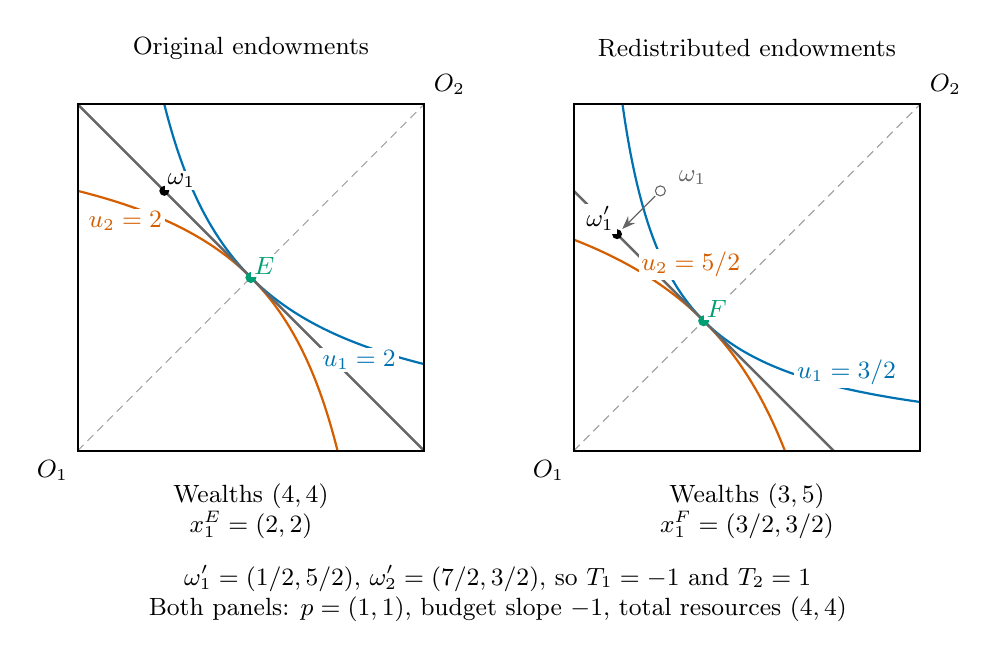
\begin{tikzpicture}[x=1.1cm,y=1.1cm,>=Stealth,font=\small]
  \begin{scope}
    \node at (2,4.65) {Original endowments};
    \draw[BookGray!60,densely dashed] (0,0)--(4,4);
    \draw[BookBlue,thick,domain=1:4,samples=120]
      plot (\x,{4/\x});
    \draw[BookOrange,thick,domain=0:3,samples=120]
      plot (\x,{4-4/(4-\x)});
    \draw[BookGray,line width=.9pt] (0,4)--(4,0);
    \draw[thick] (0,0) rectangle (4,4);
    \node[below left] at (0,0) {$O_1$};
    \node[above right] at (4,4) {$O_2$};
    \fill (1,3) circle(1.8pt)
      node[above right,fill=white,inner sep=1pt] {$\omega_1$};
    \fill[BookGreen] (2,2) circle(2pt)
      node[above right,fill=white,inner sep=1pt] {$E$};
    \node[BookBlue,fill=white,inner sep=1pt] at (3.25,1.05) {$u_1=2$};
    \node[BookOrange,fill=white,inner sep=1pt] at (.55,2.65) {$u_2=2$};
    \node[align=center] at (2,-.7)
      {Wealths $(4,4)$\\$x_1^E=(2,2)$};
  \end{scope}
  \begin{scope}[xshift=6.3cm]
    \node at (2,4.65) {Redistributed endowments};
    \draw[BookGray!60,densely dashed] (0,0)--(4,4);
    \draw[BookBlue,thick,domain=.5625:4,samples=120]
      plot (\x,{2.25/\x});
    \draw[BookOrange,thick,domain=0:2.4375,samples=120]
      plot (\x,{4-6.25/(4-\x)});
    \draw[BookGray,line width=.9pt] (0,3)--(3,0);
    \draw[thick] (0,0) rectangle (4,4);
    \node[below left] at (0,0) {$O_1$};
    \node[above right] at (4,4) {$O_2$};
    \draw[BookGray,fill=white] (1,3) circle(1.8pt);
    \node[BookGray,anchor=west] at (1.1,3.15) {$\omega_1$};
    \draw[->,BookGray] (.94,2.94)--(.56,2.56);
    \fill (.5,2.5) circle(1.8pt)
      node[above left,fill=white,inner sep=1pt] {$\omega'_1$};
    \fill[BookGreen] (1.5,1.5) circle(2pt)
      node[above right,fill=white,inner sep=1pt] {$F$};
    \node[BookBlue,fill=white,inner sep=1pt] at (3.15,.9) {$u_1=3/2$};
    \node[BookOrange,fill=white,inner sep=1pt] at (1.35,2.15) {$u_2=5/2$};
    \node[align=center] at (2,-.7)
      {Wealths $(3,5)$\\$x_1^F=(3/2,3/2)$};
  \end{scope}
  \node[align=center] at (4.85,-1.65)
    {$\omega'_1=(1/2,5/2)$, $\omega'_2=(7/2,3/2)$, so $T_1=-1$ and $T_2=1$\\
     Both panels: $p=(1,1)$, budget slope $-1$, total resources $(4,4)$};
\end{tikzpicture}
\end{document}
